\chapter{Preliminaries}\label{ch:preliminaries}

\section{Supervised Learning}\label{sec:supervised_leaning}
Supervised Learning is a well-established paradigm in machine learning where an
algorithm is trained to map input data (features) to the corresponding output
variables (targets) of a labeled dataset. The aim is to learn a model that can
predict in the best way possible the outputs of new input data. Let $\mathbf{x}
    \in \mathcal{X}$ be the input vectors (features) and $ y \in \mathcal{Y}$ be
the associated output variables (targets). The training set consists of $N$
independent and identically distributed (i.i.d.) tuples $\{(\mathbf{x_i},
    y_i)\}^N_{i=1}$ drawn from an unknown joint probability distribution
$P(\mathbf{x},y)$.

The main goal of supervised learning is to approximate the underlying
input-output relation by inducing a function $h(\mathbf{x})$, that generalizes
and can make predictions for new unseen data.

Formally given a learning model $\mathcal{L} = (\mathcal{H},\ell)$ which
includes a hypothesis space $\mathcal{H}$ and a loss function $\ell: \mathbb{R}
    \times \mathbb{R} \rightarrow \mathbb{R}$, the \textit{expected risk} of a
hypothesis $h \in H$ is defined as
\begin{equation}
    R_P(h) = \mathbb{E}_P[\ell(h(\mathbf{x}),y)] = \int_{\mathcal{X}} \int_{\mathcal{Y}}
    \ell(h(\mathbf{x}),y)P(\mathbf{x},y)dyd\mathbf{x}
\end{equation}
where $\mathbb{E}_P$ denotes the expectation with respect to the joint
The objective is to find the hypothesis $h^* \in \mathcal{H}$ that minimizes
the expected risk:
\begin{equation}
    h^* = \underset{h \in \mathcal{H}}{\arg\min} R_P(h)
\end{equation}
However, since the distribution $P(\mathbf{x},y)$ is typically unknown, the
expected risk cannot be computed directly. Instead, an empirical version is
used, based on a finite set of training samples. The \textit{empirical risk} is
computed as:
\begin{equation}
    \hat{R}_p(h) = {\frac{1}{N}} \sum^N_{i=1} \ell(h(\mathbf{x_i}),y_i)
\end{equation}
This leads to the principle of \textit{empirical risk minimization}, where the
goal is to find the hypothesis $\hat{h}$ that minimizes the empirical risk:
\begin{equation}
    \hat{h} = \underset{h \in \mathcal{H}}{\arg\min} \hat{R}_P(h)
\end{equation}

\section{Unsupervised Learning}\label{sec:unsupervised_learning}
Unsupervised learning refers to a branch of machine learning concerned with
uncovering underlying structure or patterns in a dataset without being provided
labeled outputs. In this setting, only input data $\mathbf{x} \in \mathcal{X}$
is available, typically drawn from an unknown probability distribution
$P(\mathbf{x})$, and no supervision signal (target variable) is provided.

The learning process aims to discover meaningful representations or groupings
that reveal properties of the data such as clusters, latent factors, or
manifolds. The precise goal of unsupervised learning depends on the specific
task, which may include clustering, dimensionality reduction, density
estimation, or representation learning.

Unlike supervised learning, where the risk is naturally defined with respect to
a prediction error on a known target, unsupervised learning often lacks a
unique objective function. Instead, each task introduces its own criteria:
\begin{itemize}
    \item In clustering, algorithms aim to assign data points to groups such that
          intra-cluster similarity is maximized while inter-cluster similarity is
          minimized;
    \item In dimensionality reduction, methods seek low-dimensional embeddings that
          preserve specific properties of the data, such as variance (PCA) or
          neighborhood structure (t-SNE, UMAP);
    \item In density estimation, the goal is to estimate the data-generating distribution
          $P(\mathbf{x})$ itself.
\end{itemize}

Formally, many unsupervised learning problems can be cast as a general
optimization problem of the form:
\begin{equation}
    \hat{h} = \underset{f \in \mathcal{F}}{\arg\min} \mathcal{L}(f; \mathbf{x_1,\ldots,x_N}),
\end{equation}
where $\mathcal{F}$ is the space of candidate functions or models, and
$\mathcal{L}$ is a task-specific loss function that quantifies the quality of
the learned structure (e.g., reconstruction error, likelihood, clustering
objective). Unlike in supervised learning, $\mathcal{L}$ does not directly
compare predictions to ground truth targets, but instead measures
inter-consistency or data fit.

\section{Clustering}\label{sec:clustering}

Clustering is a fundamental task in unsupervised learning that aims to
partition a dataset into groups, or \textit{clusters}, such that instances
within the same cluster are more similar to each other than to instances in
different clusters. It is a key technique for discovering underlying structure,
compressing data, detecting outliers, and analyzing patterns in
high-dimensional datasets. Formally, let

\begin{equation}
    \mathcal{D} = \{\mathbf{x}_1, \mathbf{x}_2, \ldots, \mathbf{x}_N\} \subset \mathbb{R}^d,
\end{equation}
where each $\mathbf{x}_i$ is a data point sampled from an unknown distribution
$P(\mathbf{x})$. The clustering task involves assigning each point a label $c_i
    \in \{1, \ldots, K\}$, where $K$ is either predefined, estimated automatically
or selected via model selection techniques.
A clustering $\mathcal{C} = \{C_1, C_2, \ldots, C_K\}$
must satisfy the following conditions:
\begin{equation}
    \begin{cases}
        C_k \subseteq \mathcal{D}, & \forall k \in \{1, \ldots, K\} \\
        C_i \cap C_j = \emptyset,  & \forall i \neq j               \\
        \bigcup_{k=1}^{K} C_k = \mathcal{D}
    \end{cases}
\end{equation}

Each clustering algorithm defines an objective function $\mathcal{L}$, often
representing intra-cluster similarity or inter-cluster separation. The optimal
clustering is obtained by minimizing this objective over all admissible
partitions:
\begin{equation}
    \hat{\mathcal{C}} = \underset{\mathcal{C} \in \mathbf{S}}{\arg\min} \, \mathcal{L}(\mathcal{C}; \mathcal{D}),
\end{equation}
where $\mathbf{S}$ denotes the space of valid partitions of $\mathcal{D}$.

\subsection*{Clustering Algorithms}
Clustering methods are generally categorized based on their underlying
assumptions and mechanisms, as discussed by Ezugwu et
al.~\cite{clustering_survey}:

\textbf{Partition-based Clustering:}
These algorithms divide the dataset into a set number of non-overlapping
subsets (clusters) by optimizing a specific criterion.
\begin{itemize}
    \item \emph{K-means}~\cite{k_means}: Partitions data into $k$ clusters by minimizing
          the sum of squared distances between data points and their assigned
          cluster centroid.
    \item \emph{K-medoids (PAM)}~\cite{k_medoids}: Similar to K-means but selects actual
          data points (medoids) as cluster centers, making it more robust to
          outliers.
\end{itemize}

\textbf{Hierarchical Clustering:}
These methods create a hierarchy of clusters either by progressively
merging (agglomerative) or splitting (divisive) clusters.
\begin{itemize}
    \item \emph{BIRCH}~\cite{birch}: Efficient for large datasets; incrementally
          constructs a clustering feature (CF) tree and applies clustering
          to its leaves.
    \item \emph{CURE}~\cite{cure}:  Selects well-scattered points in each cluster
          and shrinks them towards the centroid to better handle arbitrary
          shapes and outliers.
\end{itemize}

\textbf{Density-based Clustering:}
Clusters are formed based on areas of high density separated by areas
of low density, allowing detection of arbitrarily shaped clusters.
\begin{itemize}
    \item \emph{DBSCAN}~\cite{dbscan}: Groups points that are closely packed and labels
          as outliers those lying in low-density regions.
    \item \emph{OPTICS}~\cite{optics}: Extends DBSCAN by capturing the clustering structure
          at multiple density levels without a fixed threshold.
\end{itemize}

\textbf{Fuzzy Clustering:}
Unlike hard clustering, these algorithms assign each data point a membership
value for each cluster, allowing soft assignments.
\begin{itemize}
    \item \emph{Fuzzy C-Means (FCM)}~\cite{fuzzy_c_means}: Minimizes an objective function by
          allowing data points to belong to multiple clusters with varying degrees.
\end{itemize}

\textbf{Distribution-based Clustering:}
These methods assume the data is generated from a mixture of probabilistic
distributions and infer the parameters of those distributions.
\begin{itemize}
    \item \emph{Gaussian Mixture Models (GMM)}~\cite{gaussian_mixtures}: Uses the Expectation-Maximization (EM)
          algorithm to model data as a mixture of Gaussians, providing soft cluster memberships.
\end{itemize}

\textbf{Grid-based Clustering:}
These algorithms divide the data space into a finite number of grid cells
and perform clustering on the grid structure.
\begin{itemize}
    \item \emph{CLIQUE}~\cite{clique}: Combines grid-based and density-based methods
          to efficiently identify clusters in high-dimensional data.
\end{itemize}

\textbf{Model-based Clustering:}
These approaches assume a model for each cluster and optimize the fit of the model to the data.
\begin{itemize}
    \item \emph{Self-Organizing Maps (SOM)}~\cite{som}: A type of neural network that
          maps high-dimensional input data into a lower-dimensional (typically 2D)
          representation while preserving topological relationships.
\end{itemize}

\subsection*{Clustering Evaluation Metrics}

Clustering evaluation metrics are broadly classified into \textbf{internal} and
\textbf{external} criteria. Internal metrics assess the quality of a clustering
using only the input data and the clustering result, without reference to any
external information. External metrics, on the other hand, require ground truth
labels to compare the clustering against known class memberships.

\textbf{Silhouette Coefficient:} This metric measures how similar a data point is to
its own cluster compared to other clusters. For a data point $i$, the silhouette score
is defined as:
\begin{equation}
    s(i) = \frac{b(i) - a(i)}{\max\{a(i), b(i)\}},
\end{equation}
where $a(i)$ is the average distance from $i$ to all other points in its
cluster, and $b(i)$ is the smallest average distance from $i$ to points in a
different cluster. The coefficient ranges from $-1$ to $1$, where values close
to $1$ indicate well-clustered points.

\textbf{Davies-Bouldin Index (DBI):} This metric evaluates the average similarity between each
cluster and its most similar cluster, defined as the sum of the within-cluster distances divided
by the between-cluster centroid distances. Formally:
\begin{equation}
    \text{DBI} = \frac{1}{K} \sum_{i=1}^{K} \max_{j \ne i} \left( \frac{\sigma_i + \sigma_j}{d_{ij}} \right),
\end{equation}
where $\sigma_i$ is the average distance of points in cluster $i$ to its
centroid, and $d_{ij}$ is the distance between the centroids of clusters $i$
and $j$. Lower values of DBI indicate better clustering.

\textbf{Adjusted Rand Index (ARI):} The ARI compares the similarity between the predicted clusters
and the ground truth labels, correcting for chance groupings:
\begin{equation}
    \text{ARI} = \frac{\text{RI} - \mathbb{E}[\text{RI}]}{\max(\text{RI}) - \mathbb{E}[\text{RI}]},
\end{equation}
where $\text{RI}$ is the Rand Index and $\mathbb{E}[\text{RI}]$ is its expected
value under random assignments. ARI values range from $-1$ to $1$, with $1$
indicating perfect agreement.

\textbf{Normalized Mutual Information (NMI):} NMI measures the amount of shared information
between the clustering assignments and the ground truth labels:
\begin{equation}
    \text{NMI}(U, V) = \frac{2 \cdot I(U; V)}{H(U) + H(V)},
\end{equation}
where $I(U; V)$ is the mutual information and $H(\cdot)$ denotes entropy. NMI
ranges from $0$ (no mutual information) to $1$ (perfect correlation), and is
particularly useful when the number of clusters differs from the number of
classes.

Each metric provides a different perspective on clustering quality. Internal
metrics are essential when no labels are available, while external metrics
offer direct validation against known structure in labeled datasets.

\section{Stream Learning}\label{sec:stream_learning}
In many real-world applications, data is not available as a static, finite
dataset but rather arrives continuously over time in the form of a stream.
Stream Learning, also known as Online Learning or Incremental Learning, is a
machine learning paradigm designed to handle such continuously evolving data
environments. Unlike traditional batch learning methods, stream learning
algorithms are capable of processing data points individually or in small
batches, often in a single pass, and updating their models incrementally.

Formally, let $\{\mathbf{x_1, x_2,\ldots} \} $ be a potentially infinite
sequence of data points drawn from a stream. The stream learning algorithm
maintains a model $\mathcal{M}_t$ at each time step $t$ which is updated upon
receiving a new data point $\mathbf{x}_t$. The update is performed using a
function $U$ such that:
\begin{equation}
    \mathcal{M}_{t+1} = U(\mathcal{M}_t, \mathbf{x_t})
\end{equation}
This formulation enables the model to adapt continuously over time while
operating within bounded memory and computational constraints, as required
in streaming scenarios where incoming data can be potentially infinite.

This paradigm poses unique challenges, particularly in maintaining stability
while adapting to new information and detecting changes in the underlying data
distribution.

\section{Explainability in Machine Learning}\label{sec:explainability}

Explainability in Machine Learning refers to the capacity to understand and
interpret the internal mechanics or predictions of a model. As machine learning
systems are increasingly deployed in high-stakes domains such as healthcare,
finance, and autonomous systems, understanding how and why decisions are made
is essential for building trust, ensuring accountability, and complying with
ethical or legal standards~\cite{importance_of_explainabilty}.

Some models are inherently interpretable such as decision trees, linear
regression, and logistic regression where the influence of each feature is
explicitly encoded in the model's structure or coefficients. For example, in
linear models, the prediction for an instance $x \in \mathbb{R}^d$ is given by:
\begin{equation}
    \hat{y} = w^\top x + b,
\end{equation}
where each coefficient $w_i$ directly indicates the contribution of feature
$x_i$ to the prediction.

However, many high-performing models such as deep neural networks (DNNs),
support vector machines (SVMs), and ensemble methods like Random Forests and
Gradient Boosting Machines are considered \emph{black boxes} due to their
complexity and lack of direct interpretability.

To address this, a variety of \emph{post-hoc} interpretability techniques have
been developed. These can be broadly categorized into global (model-level) and
local (prediction-level) explanations.

One widely used approach is \textbf{feature importance}, which quantifies the
contribution of each input feature to the model's overall performance:

\begin{itemize}
    \item In tree-based ensamble models, feature importance is often computed by summing the
          decrease in impurity (e.g., Gini index or entropy) resulting from splits on
          that feature across all trees: \begin{equation} \text{Importance}(f_i) =
              \sum_{t \in T} \sum_{s \in \text{Splits}(t, f_i)} \Delta \text{Impurity}(s),
          \end{equation}
          where $T$ is the set of trees in the ensemble, and $s$ are the split points
          involving feature $f_i$.

    \item In \textbf{permutation importance}, the values of feature $f_i$ are randomly
          permuted to break the association with the target, and the drop in performance
          (e.g., accuracy or $R^2$) is recorded:
          \begin{equation} \text{Importance}_{\text{perm}}(f_i) =
              \mathcal{M}(\mathcal{D}) - \mathcal{M}(\mathcal{D}_{\pi_i}),
          \end{equation}
          where $\mathcal{M}(\cdot)$ is the model evaluation metric and
          $\mathcal{D}_{\pi_i}$ denotes the dataset with feature $f_i$ permuted.
\end{itemize}

\textbf{Local interpretability} methods explain individual predictions by approximating
the decision boundary around a specific input:

\begin{itemize}
    \item \textbf{LIME} (Local Interpretable Model-agnostic Explanations)~\cite{lime} fits a
          simple surrogate model (usually linear) around the neighborhood of the instance $x$ by
          minimizing a weighted loss:
          \begin{equation}
              \mathcal{L}(f, g, \pi_x) = \sum_{z \in \mathcal{Z}} \pi_x(z) (f(z) - g(z))^2 + \Omega(g),
          \end{equation}
          where $f$ is the original model, $g$ is the interpretable surrogate, $\pi_x(z)$
          is a locality-aware kernel, and $\Omega(g)$ penalizes model complexity.

    \item \textbf{SHAP} (SHapley Additive exPlanations)~\cite{shap} assigns each feature an
          additive contribution to the prediction based on Shapley values from cooperative game theory:
          \begin{equation}
              f(x) = \phi_0 + \sum_{i=1}^{d} \phi_i,
          \end{equation}
          where $\phi_0$ is the expected model output and $\phi_i$ quantifies the
          contribution of feature $i$ to the prediction. SHAP values are uniquely
          characterized by properties such as \textit{local accuracy},
          \textit{missingness}, and \textit{consistency}.
\end{itemize}

These tools help practitioners better understand, trust, and debug machine
learning models. As machine learning continues to permeate real-world
applications, explainability will remain a cornerstone of responsible AI
development.

\section{Data Drift}\label{sec:data_drift}
Data drift refers to the phenomenon where the statistical properties of data
change over time. This can lead to reduced model performance if the model is
not adapted to the evolving data distribution. In real-world applications, the
concept of drift is often encountered due to changing environments, user
behavior, or external factors. Addressing data drift is crucial for maintaining
the reliability and accuracy of machine learning models over time. Drift can
occur in various forms, such as changes in the input data (input drift), in the
target labels (prediction drift), or in the underlying relationships between
the data and the target (concept drift). Detecting and adapting to data drift
is an essential part of maintaining long-term model performance.

\subsection*{Drift Definitions}\label{subsec:drift_definitions}
Following the definitions provided by Gama et
al.~\cite{drift_adaptation_survey}, this section outlines formal definitions of
\textbf{concept drift} and its key variants.

Concept drift is said to occur between two time points $t_0$ and $t_1$ if:
\begin{equation}
    \exists X : p_{t_0}(X, y) \neq p_{t_1}(X, y)
\end{equation}
where $p_t(X, y)$ represents the joint distribution of the input variables $X$
and the target variable $y$ at time $t$.

This change in the joint distribution can be decomposed into the following
components:
\begin{itemize}
    \item A shift in the prior distribution of the target variable: $p(y)$,
    \item A change in the class-conditional distribution of the inputs: $p(X \mid y)$,
    \item A resulting shift in the posterior distribution: $p(y \mid X)$.
\end{itemize}

From the perspective of predictive modeling, two principal types of concept
drift are commonly distinguished:

\begin{enumerate}
    \item \textbf{Real Concept Drift}: Defined as a change in the posterior
          distribution over time:
          \begin{equation}
              p_{t_0}(y \mid X) \neq p_{t_1}(y \mid X)
          \end{equation}
          This type of drift affects the underlying decision function.

    \item \textbf{Virtual Concept Drift}: Occurs when the marginal distribution
          of the input features changes while the posterior distribution remains stable:
          \begin{equation}
              p_{t_0}(X) \neq p_{t_1}(X) \quad \text{and} \quad p_{t_0}(y \mid X) =
              p_{t_1}(y \mid X)
          \end{equation}
          Although the optimal predictive function remains unchanged, this form
          of drift may still impact performance through mechanisms such as covariate
          shift, sampling bias, or changes in feature relevance.
\end{enumerate}

From a model maintenance perspective, only changes in the posterior distribution $p(y \mid X)$—as
seen in real concept drift—have a direct impact on the predictive function and thus
necessitate adaptation or retraining. In contrast, virtual drift, while potentially
affecting performance indirectly, does not alter the relationship between inputs and
outputs and may not always require immediate corrective measures.

\begin{figure}[h]
    \centering
    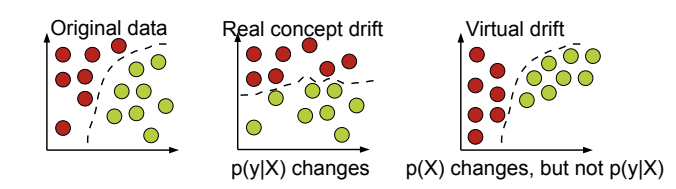
\includegraphics[width=1\textwidth]{my_images/drift_types.png}
    \caption{Types of concept drift. Source:~\cite{drift_adaptation_survey}}\label{fig:concept_drift_types}
\end{figure}

Although real concept drift is formally defined by changes in $p(y \mid X)$, in
practice, such changes may manifest through observable shifts in the marginal
input distribution $p(X)$, particularly when certain input regions become more
prevalent or undergo structural changes. As a result, analyzing how $p(X)$
evolves over time can offer valuable insights into the nature and causes of
concept drift—even when true labels are unavailable.

\subsection*{Drift Detection}\label{subsec:drift_detection}
Concept drift detection identifies changes in the statistical properties of
data streams that affect model performance. A typical framework consists of
four main stages~\cite{learning_under_concept_drift}:

\begin{enumerate}
    \item \textbf{Data Retrieval}: Organizes incoming data into chunks
          suitable for analysis.
    \item \textbf{Data Modeling (Optional)}: Transforms or reduces the data
          for efficiency or interpretability.
    \item \textbf{Test Statistic Computation}: Quantifies differences between
          past and current data or model performance.
    \item \textbf{Hypothesis Testing}: Determines whether detected differences
          are statistically significant.
\end{enumerate}

These stages are common across most detection algorithms and support flexible
implementation across streaming scenarios.

Drift detection algorithms can be broadly categorized into three groups based
on the nature of their test statistics.

\textbf{Error-Rate-Based Methods} monitor the performance of a predictive model.
A significant increase in error rate suggests concept drift.
Notable algorithms include:

\begin{itemize}
    \item \emph{DDM} (Drift Detection Method)~\cite{ddm}: Detects drift when the
          classification error increases beyond statistical thresholds.
    \item \emph{EDDM}~\cite{eddm}: Improves DDM by considering the distance between errors,
          making it more sensitive to gradual drifts.
    \item \emph{ADWIN}~\cite{adwin}: Maintains a variable-length window and compares
          statistics between subwindows.
\end{itemize}

\textbf{Distribution-Based Methods} compare statistical properties of data distributions directly,
often in an unsupervised setting.

\begin{itemize}
    \item \emph{LSDD}~\cite{lsdd}: Uses a kernel-based method to measure the difference
          between distributions.
    \item \emph{ITA}~\cite{ita} (Information-Theoretic Approach): Relies on entropy and divergence
          measures to detect distributional changes.
    \item \emph{SyncStream}~\cite{syncstream}: Captures synchronized structural changes in multidimensional streams.
\end{itemize}

\textbf{Ensemble and Multi-Test Methods} use multiple statistical tests or detectors in parallel or
hierarchically to improve robustness and adaptivity.

\begin{itemize}
    \item \emph{JIT} (Just-in-Time Drift Detection)~\cite{jit}: Tests various feature combinations
          for localized drift detection.
    \item \emph{HHT} (Hierarchical Hypothesis Testing)~\cite{hht}: Combines quick detection with
          secondary validation to reduce false alarms.
    \item \emph{e-Detector}~\cite{e_detector}: Leverages an ensemble of heterogeneous detectors to
          balance early detection and accuracy.
\end{itemize}

Each category addresses different aspects of the drift detection problem.
Error-rate-based methods are tightly coupled with the model but rely on labeled
data. Distribution-based methods are model-agnostic and can work without
labels, while ensemble and hierarchical approaches aim to improve detection
reliability under varying conditions.

\subsection*{Drift Adaptation}\label{subsec:drift_adaption}

Concept drift adaptation refers to the broad set of techniques designed to
maintain predictive performance in the presence of changing data distributions.
This field is commonly referred to as \emph{Adaptive Learning}.

Gama et al.~\cite{drift_adaptation_survey} classify adaptation strategies into
two primary categories:

\begin{enumerate}
    \item \textbf{Blind methods}: These methods adapt the model continuously or
          periodically, without relying on explicit drift detection mechanisms.
          They are typically simpler and more responsive but may incur unnecessary
          updates when no drift has occurred.
    \item \textbf{Informed methods}: These approaches rely on the output of drift
          detectors to guide the adaptation process. By updating the model only when drift
          is detected, they aim to achieve more efficient and targeted adaptation.
\end{enumerate}

An alternative taxonomy proposed by Lu et
al.~\cite{learning_under_concept_drift} focuses on how the model is updated:

\begin{itemize}
    \item \textbf{Simple retraining}: Upon detection of concept drift, the
          current model is discarded and a new one is trained using the most recent
          data. A sliding or adaptive window is often used to select relevant training
          samples.
    \item \textbf{Model adjusting}: Instead of retraining the entire model,
          only affected parts are incrementally updated. This approach is particularly
          effective for handling localized or gradual drift, and is generally more
          efficient.
    \item \textbf{Ensemble retraining}: Rather than relying on a single model,
          ensemble methods maintain a pool of base classifiers. Adaptation is achieved
          by updating, weighting, replacing, or adding classifiers in response to drift,
          making them especially well-suited for handling recurring or complex drifts.
\end{itemize}

The effectiveness of drift adaptation methods depends on the characteristics of
the data stream, such as the type and frequency of drift. A well-designed
adaptive system often combines both detection and adaptation mechanisms to
ensure timely and efficient responses to changes in data distribution.

\subsection*{Drift Explainability}\label{subsec:drift_explainability}

Drift explainability focuses on understanding the causes and nature of changes
in data distributions that affect machine learning models. While detecting
drift is important, it is equally critical to explain why and how drift occurs.
This understanding provides valuable insights into the model's evolving
behavior and informs decisions about retraining and maintenance.

There are several techniques for explaining drift, each aiming to reveal how
data shifts influence model behavior. One common approach involves identifying
which features have changed significantly over time and assessing how these
changes impact the model's predictions. For example, feature importance
analysis can be used to compare a model $f_{\text{ref}}$ trained on reference
data $S_P \sim P^n$ with a model $f_{\text{prod}}$ trained on production data
$S_Q \sim Q^m$. Let $\phi_i^{\text{ref}}$ and $\phi_i^{\text{prod}}$ denote the
importance of feature $i$ in the respective models. A large shift
\begin{equation}
    \Delta \phi_i = \left| \phi_i^{\text{ref}} - \phi_i^{\text{prod}} \right|
\end{equation}
may indicate that feature $i$ has changed its predictive relationship with the target.
We refer to this method as \emph{feature importance for drift explainability}.

Another powerful approach to drift explainability frames the detection of
distributional shift as a binary classification problem between the reference
dataset $S_P$ and the production dataset
$S_Q$~\cite{revisiting_two_sample_classifier}. This method—known as a
\emph{Classifier Two-Sample Test} (C2ST)—labels samples from $P$ with class 0
and samples from $Q$ with class 1, and trains a binary classifier $f:
    \mathcal{X} \rightarrow \{0, 1\}$ to distinguish between them.

If the null hypothesis $H_0: P = Q$ holds, then the classification accuracy of
$f$ on a held-out validation set $S_{\text{test}}$ should remain close to
chance level, i.e., $\text{Acc}(f) \approx 0.5$. The test statistic is given
by:
\begin{equation}
    \text{C2ST}(f) = \frac{1}{|S_{\text{test}}|} \sum_{(x, y) \in S_{\text{test}}} \mathbb{1}\{f(x) = y\}.
\end{equation}
A significant deviation from $0.5$ suggests that $P \neq Q$, indicating distributional drift.

Beyond detection, C2STs offer an interpretable means to explain drift by
examining the feature importances of the trained classifier. This technique,
referred to as \emph{concept feature importance for drift explainability},
highlights which features $x_i$ contribute most to $f(x)$, and hence to the
difference between $P$ and $Q$.

Understanding the factors behind drift is essential for effective model
management. Without explainability, decisions about retraining may be based on
guesswork, potentially leading to unnecessary updates or degraded performance.
Drift explainability ensures that model updates are both necessary and
well-targeted, guided by principled statistical and model-based insights.